\chapter{LHC and ATLAS}
\label{chap:cern}

The analyses presented in this thesis use the data collected by the ATLAS experiment in 2015, 2016 and 2017 at \cmtre TeV; the ATLAS experiment is one of the four main experiments at the Large Hadron Collider (LHC) at CERN. Section \ref{sed:cern:lhc} of this chapter describes the LHC accelerator complex, followed by a description of the ATLAS detector in Section \ref{sed:cern:atlas}.

%%%%%%%%%%%%%%%%%% LHC

\section{The Large Hadron Collider}
\label{sed:cern:lhc}

In this section we give a brief introduction to the Large Hadron Collider (LHC) \cite{1748-0221-3-08-S08001}, at the moment the largest and most powerful particle accelerator in the world, hosted by the European Organization for Nuclear Research (CERN) and active since September 2008.



\subsection{A Circular Hadron Collider}

The LHC is a circular hadron accelerator, located in a 26.7-km-long underground tunnel (with a depth ranging between 50 and 140 meters) that was previously hosting the Large Electron-Positron Collider (LEP), a CERN accelerator active from 1989 to 2000. The LHC can accelerate protons up to a design center-of-mass energy of 7 TeV. Accelerating particles to very high energies is necessary to both study the structure of the particles themselves at smaller scales, and to create heavy states in collisions. Cosmic rays provide a source of particles with energies up to $10^7$ times more than what the LHC is capable of, but these extremely energetic rays are very rare, and the flux is not controlled. Accelerators provide a well controlled flux of particles of a specific type in a specific location, and this allows the study of these particles with dedicated detectors.

A circular accelerator simplifies the acceleration of the particles, as this can happen over several revolutions. When a charged particle travels on an orbit of radius r under the effect of a magnetic field B, its momentum p is given by:
\begin{equation}
\label{eq:cern:p03br}
p = 0.3 B r,
\end{equation}
\noindent where the momentum is expressed in GeV, B in Tesla and the radius of the orbit in meters. For a given magnetic field, a larger radius allows to reach higher energies. 

The choice of a collider over a fixed-target experiment is motivated by the possibility of reaching an higher energy in the center of mass system: while in a fixed-target experiment this is proportional to the square root of the incoming particle, in a collider is the sum of the energies of the two beams.


Suitable particles for a collider experiment need to fulfill two criteria: they need to be charged, in order to be accelerated and guided through electric and magnetic fields, and they need to be stable enough not to decay before being used for collisions. These criteria effectively limit the choice to protons, electrons and their antiparticles, in addition to ions. 

At the LHC it has been chosen to study collisions with protons and lead ions. Three types of collisions are studied: proton-proton ($p-p$), lead-lead ($Pb-Pb$) and also proton-lead ($Pb-p$). The main reason to prefer protons over electrons is the energy loss that affects charged particles accelerated in a circular trajectory (\textit{syncrotron radiation}), that decreases with the fourth power of the mass of the particle:

\begin{equation}
\label{eq:cern:sync}
\frac{dE}{dt} \propto \frac{E^4}{m^4 r}
\end{equation}

The larger mass of a proton with respect to an electron leads to a decrease of a factor $10^{12}$ of the energy lost for syncrotron radiation. This choice comes with a price: proton-proton collisions lead to less clean events, where a lot of soft interactions covering the interesting hard interactions and the center of mass is unknown as the particles taking part in hard interactions are not the protons themselves but their constituents.

\subsection{Magnet System} 


The LHC is not a perfect circumference: it is composed by eight arcs (\textit{sectors}), where the magnetic system is located, and eight straight sections containing the resonant cavities, the detectors, the equipment for beam injection and extraction, and other instrumentation. Magnetic fields are used to govern the trajectory of the particles. In the LHC there are more than nine thousand magnets, constructed from a superconducting alloy of niobium and titanium. 150 tons of super-fluid helium at the temperature of 1.9 K are used to maintain the magnet system in the superconducting regime. The different types of magnets necessary to achieve a proper control over the trajectory of the particles are:

\subsubsection*{Dipoles} 
Dipoles are used to create a vertical magnetic field, to bend the particles in the horizontal plane and give the dominant circular orbit. The LHC has 1232 dipoles, each 15 m long and providing a magnetic field of 8.3 T. The current necessary to achieve this strong magnetic field is 11.8 kA.


\subsubsection*{Quadrupoles}
The LHC has 858 quadrupoles, used for beam focusing. A single quadrupole can focus the beam either in the vertical or horizontal plane, but causes a defocusing on the other; conventionally a quadrupole is denoted as focusing if it is oriented to focus in the horizontal plane. A combination of focusing and defocusing quarupoles separated by some drift space (\textit{FODO lattice}) is used to keep both planes focused, and gives rise to \textit{Betatron oscillations}. Fig. \ref{fig:lhc:quad} shows a schematic representation of the transverse view of a quadrupole magnet.

\subsubsection*{Higher-order Magnets} 
Beside dipoles and quadrupoles, in the LHC there are about 600 higher-order magnets are used to maintain a good beam quality; for example sextupoles are used to correct the spread in Betatron tune caused by the quadrupoles.




\begin{figure}[ht]
\centering
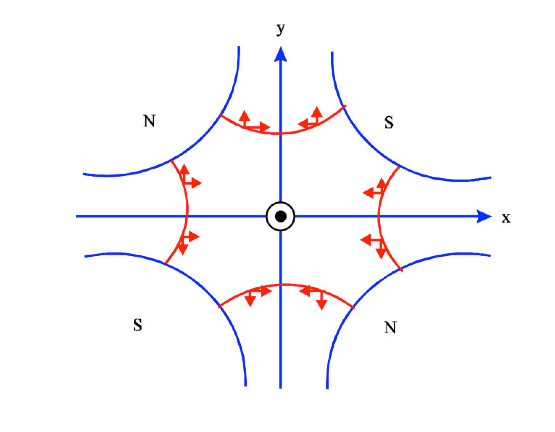
\includegraphics[width=0.45\textwidth]{figures/lhc/figures_quad}
\caption{A schematic cross-section of a quadrupole magnet. The red arrows indicate the direction of the force on the particle. Figure from Ref. \cite{Kain:2016aly}.}
\label{fig:lhc:quad}
\end{figure}

\subsection{Resonant Cavities}

While the orbit of the particles is governed through magnetic fields, longitudinal electric fields are used for acceleration. In the LHC the electric filed is provided by the \textit{radiofrequency (RF) cavities}. There are overall 16 RF cavities, 8 per beam, hosted in four cryo-modules. Each cavity can create a field up to 2 MV (providing an accelerating field of 5 MV/m), and oscillates with a frequency of 400 MHz. Since the electric field changes over time with the oscillations, particles passing through the same point of a RF cavity in different moments experience a different voltage; this produces a non-trivial longitudinal dynamic, where particles oscillates around the ideal synchronous particle with changes is momentum and phase (\textit{Synchrotron oscillations}). If we define the \textit{slip factor} $\eta$ as the relative change in frequency in Synchrotron oscillations with the relative change in momentum:
\begin{equation}
\eta = \frac{\Delta f / f}{\Delta p / p}
\end{equation}

and the compaction factor $\alpha$ as the relative change in frequency in orbit length with the relative change in momentum:

\begin{equation}
\eta = \frac{\Delta L / L}{\Delta p / p} \; ,
\end{equation}

the following relation holds:
\begin{equation}
\eta = \frac{1}{\gamma^2} - \alpha \; ,
\end{equation}

where $\gamma$ is the Lorentz factor of the particle. This means that while the energy of the particle is low ($\eta>0$) an increase in momentum leads to an increase in frequency, while it leads to a decrease in frequency for $\eta<0$. At the transition energy a previously stable synchrotron phase becomes unstable and vice versa; this requires a rapid change in RF phase. This situation is illustrated in Fig. \ref{fig:lhc:phase}(a). For example, a particle corresponding to the phase point M1 will arrive in the RF cavity after one corresponding to the stability point P1, and will experiment higher voltage and increase in momentum; if $\eta>0$ this increase in momentum will translate in an increase in frequency and the particle will, at the following revolution, arrive earlier, while if $\eta<0$ the frequency will further decrease and the particle will be eventually lost.  The transition energy in the LHC is 53 GeV, well below the injection energy of 450 GeV, so the LHC is always above transition. 

\begin{figure}[ht]
\centering
\subfigure{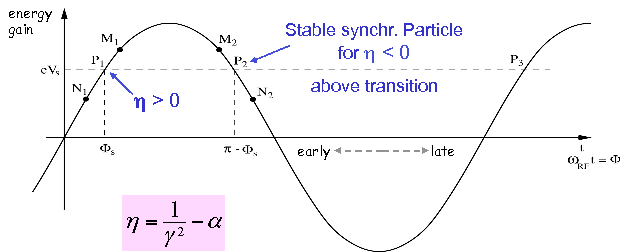
\includegraphics[width=0.547\textwidth]{figures/lhc/phase-stability-2}}
\subfigure{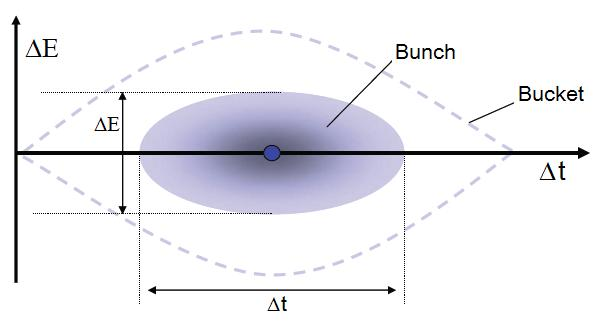
\includegraphics[width=0.44\textwidth]{figures/lhc/bucket}}
\caption{(a) Phase stability below and above transition. Figure from Ref. \cite{Tecker:2016mlq}. (b) Bucket and the bunch area.}
\label{fig:lhc:phase}
\end{figure}

The areas of stable motion are identified as \textit{bucket}, and the area of the bucket is the beam \textit{longitudinal acceptance}. The beam bunches fill only a part of the bucket, and the area of the beam bunches is the \textit{longitudinal beam emittance}. Fig. \ref{fig:lhc:phase}(b) shows a schematic view of the bucket and the bunch area.

\subsection{Operational Parameters}

\begin{equation}
\label{eq:cern:nev}
N_{ev} = \sigma \,\, \mathcal{L}_{int}
\end{equation}

The integrated luminosity is the time integral of the instantaneous luminosity $\mathcal{L}$, 

\begin{equation}
\label{eq:cern:intlumi}
\mathcal{L}_{int} = \int \mathcal{L} \, dt
\end{equation}

which in turn is defined as:

\begin{equation}
\label{eq:cern:lumi}
\mathcal{L}=\frac{f n_1 n_2}{4 \pi \sigma_x \sigma_y}
\end{equation}


In eq. \ref{eq:cern:lumi}:
\begin{itemize}
\item f is the revolution frequency
\item $n_1$ and $n_2$ are the number of particle in each beam
\item $\sigma_x$ and $\sigma_y$ are the x and y dimensions of the beam at the interaction point
\end{itemize}


\subsection{Accelerator Complex}

\begin{itemize}
\item Linac
\item PS Booster
\item PS
\item SPS
\end{itemize}

\begin{figure}[ht]
\centering
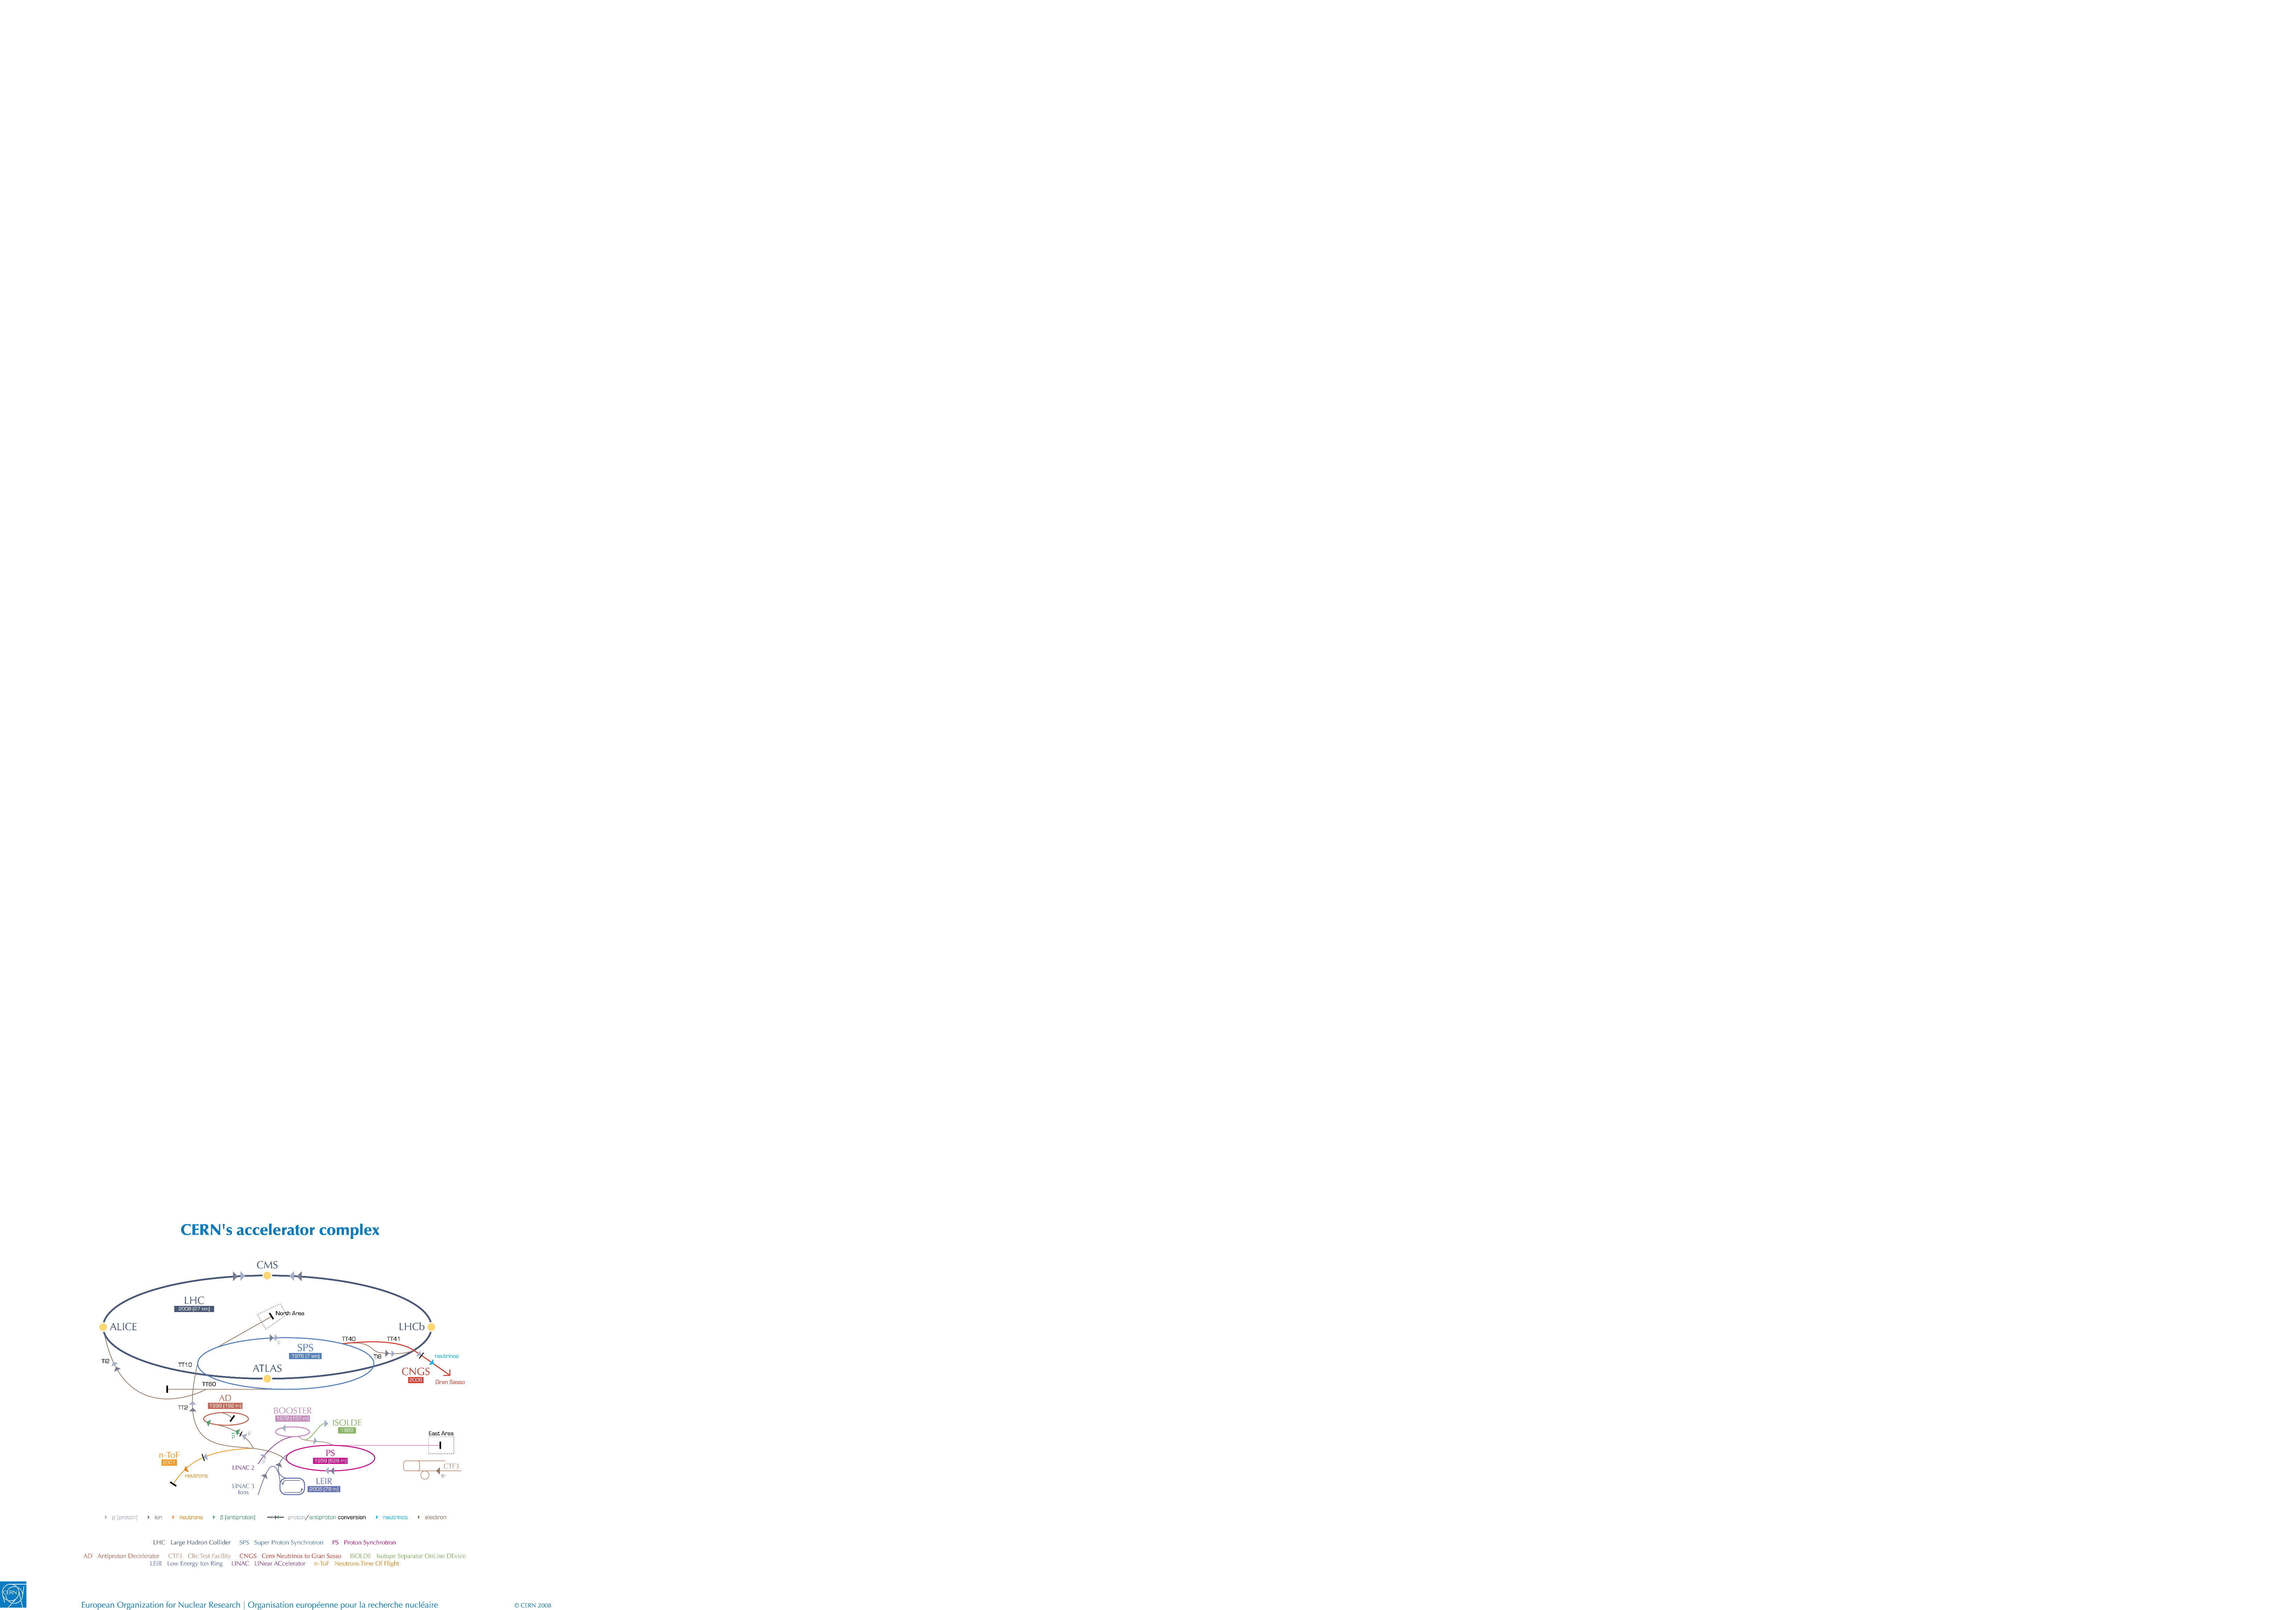
\includegraphics[width=1\textwidth]{figures/lhc/acc_complex.pdf}
\caption{CERN accelerator complex \cite{Christiane:1260465}.}
\label{fig:lhc:acc}
\end{figure}

\subsection{Experiments at the LHC}

\subsubsection*{ALICE}

\subsubsection*{CMS}

\subsubsection*{LHCb}

\subsubsection*{LHCf}

\subsubsection*{TOTEM}

\subsubsection*{ALICE}

\subsubsection*{MoEDAL}


%%%%%%%%%%%%%%%%%% ATLAS

\section{The ATLAS Experiment}
\label{sed:cern:atlas}

\subsection{Coordinate System}

\begin{equation}
\label{eq:cern:eta}
\eta = - \ln \tan \frac{\theta}{2}
\end{equation}

\begin{equation}
\label{eq:cern:y}
y = \frac{1}{2} \ln \frac{E + p_z}{E - p_z}
\end{equation}

\begin{equation}
\label{eq:cern:pt}
p_T = \sqrt{p_x^2 + p_y^2}
\end{equation}

\begin{equation}
\label{eq:cern:pz}
p_z = p_T \,\sinh \eta
\end{equation}

\begin{equation}
\label{eq:cern:dR}
\Delta R = \sqrt{ \Delta \phi^2 + \Delta \eta^2  }
\end{equation}




\subsection{Magnet System}
\label{sec:cern:atlasmagnets}

\subsubsection*{Solenoid}

\subsubsection*{Toroids}



\subsection{Inner Detector}

\subsubsection*{IBL}

\subsubsection*{Pixel Detector}


\subsubsection*{Semi-Conductor Tracker}


\subsubsection*{Transition Radiation Tracker}



\subsection{Calorimeters}

\subsubsection*{Electromagnetic Calorimeter}


\subsubsection*{Hadronic Calorimeter}


\subsubsection*{Forward Calorimeter}


\subsection{Muon Spectrometer}


\subsection{Forward Detectors}

\subsection{Trigger System}
\label{sec:cern:trigger}

\subsection{ATLAS Performance Summary}


\subsection{ATLAS Physics Program}